% \documentclass[11pt]{article}
% \usepackage[T1]{fontenc}
% \usepackage[utf8]{inputenc}
% \usepackage{microtype}
% \usepackage[margin=1in]{geometry}
% \usepackage{booktabs}
% \usepackage{longtable}
% \usepackage{array}
% \usepackage{ragged2e}
% \usepackage{caption}
% \usepackage{hyperref}
% \usepackage{pdflscape}
% \captionsetup[table]{skip=6pt}

% Paragraph-like column type with ragged-right
\newcolumntype{P}[1]{>{\RaggedRight\arraybackslash}p{#1}}

% \begin{document}
\begin{landscape}
\section*{Supplemental material}



\begin{longtable}{@{}P{2.cm} P{3.cm} P{3.cm} P{3.cm} P{2.cm} P{2.5cm} P{2.5cm} P{3.cm}@{}}
\caption{Previous models for terrain/surface classification using wearable and related sensors}\label{tab:prev-models}\\
\toprule
\textbf{Paper} & \textbf{Participants} & \textbf{Surfaces (categorized)} & \textbf{Instrumentation} & \textbf{Model(s)} & \textbf{Evaluation} & \textbf{Metrics} & \textbf{Notes / Setting} \\
\midrule
\endfirsthead
\toprule
\textbf{Paper} & \textbf{Participants} & \textbf{Surfaces (categorized)} & \textbf{Instrumentation} & \textbf{Model(s)} & \textbf{Evaluation} & \textbf{Metrics} & \textbf{Notes / Setting} \\
\midrule
\endhead
\bottomrule
\endfoot
\midrule
\multicolumn{8}{r}{\emph{Table~\ref{tab:prev-models} continued on next page}}\\
\midrule
\endfoot

% ===== IMU-only block =====
\multicolumn{8}{l}{\textbf{IMU-only}}\\
\addlinespace
Shah et al.~\cite{Shah_2022} & Luo dataset: 30 healthy adults (23.5 $\pm$ 4.2 y) & urban flat; incline/decline; stairs; natural uneven; banked & IMUs: wrist; L5; anterior thigh (bilateral); anterior shank (bilateral); models per sensor and all sensors & FNN & random and subject-wise & F1: 0.78 (subject-wise; lower limbs/trunk; right shank) 0.97 (random split; lower limbs) & Highly segmented straight-line walking data. \\
\addlinespace
Hu et al.~\cite{Hu_2021} & 17 older (71.5 $\pm$ 4.2 y) + 18 younger (27.0 $\pm$ 4.7 y) & lab brick paths (flat vs uneven) & IMU at L5--S1 & LSTM & random \(\dagger\) & Acc: 0.963 & Data leakage: same-subject data in train/test. \\
\addlinespace
Dixon et al.~\cite{dixon2019machine} & 29 young healthy (15 male), 23.3 $\pm$ 3.6 y & field mixed: road; track; trail & Accelerometers at L3--L5 (lower back) and right tibia; configs: 2-sensor; lower-back; tibia & GBoost; CNN & random 90/10 \(\dagger\) & Acc: 95.5 ($\pm$1.0) two-sensor; 94.1 ($\pm$3.8) tibia & Running; same-subject data in train/test. \\
\addlinespace
Chen et al.~\cite{chen2020determining} & 30 healthy (15 women), 24.0 $\pm$ 1.1 y & urban flat; incline/decline; stairs & IMU on exterior left shoe & CNN & random split \(\dagger\) & Acc: DL 87.74; custom 84.02 & --- \\
\addlinespace
Hashmi et al.~\cite{hashmi2019lies} & 40 (10 female) healthy young (29.2 $\pm$ 11.4 y) & urban hard vs soft (concrete/asphalt/tiles vs carpet/grass/soil) & Two smartphones: chest and lower back & RF; SVM & k-fold (no subject stratification) \(\dagger\) & Acc: 86.8 (lower-back SVM) & Likely leakage (no subject stratification). \\
\addlinespace
McGuire et al.~\cite{mcquire2021uneven} & Luo dataset: 30 healthy adults (23.5 $\pm$ 4.2 y) & urban flat; natural uneven; incline/decline; banked; stairs & IMUs: trunk; wrist; R/L thigh; R/L shank & Centralized vs decentralized (federated) ML & random 80/20 \(\dagger\) & Acc: 94.252 (SVM centralized); 88.098 (realistic federated) & Highly segmented straight-line walking data; methods uncertain. \\
\addlinespace
Ng et al.~\cite{ng2022machine} & 12 healthy (4 females) & irregular vs regular (grass; obstructions; uneven; debris) & 3D accelerometer at head; lower back; outer shoe & five classifiers & LOSO (best sensor location) \(\ddagger\) & AUC: 0.80 (right ankle, SVM) & --- \\
\addlinespace
Chauhan et al.~\cite{chauhan2025classifying}& Luo dataset: 30 healthy adults (23.5 $\pm$ 4.2 y) & urban flat; incline/decline; stairs; natural uneven; banked & IMUs: wrist; L5; anterior thigh (bilateral); anterior shank (bilateral); & VM, ANN and LightGBM with salp swarm algorithm & random\(\dagger\) & LightGBM ACC: 99.47\% & --- \\
\addlinespace
Kobayashi et al.~\cite{kobayashi2019estimation} & 7 participants & asphalt; gravel; lawn; grass; sand; mat (snow mimic) & smartphone (location unspecified) & RF & LOSO / LOSO-session & Acc: 44.9 (subject-CV \(\ddagger\)); 83.5 (session-CV) & --- \\
\addlinespace
Worsey et al.~\cite{worsey2021automatic} & 6 healthy (2 female) & athletics track; soft sand; hard sand & ankle-worn inertial sensor & SVM; XGB; LR; RF; MLP-NN & LOSO (athlete-independent) \(\ddagger\); random 70/30 (athlete-dependent) \(\dagger\) & Acc: 0.67 $\pm$ 0.17 (best LOSO SVM); 1.0 (athlete-dependent GSVM) & --- \\
\addlinespace
Bunker et al.~\cite{bunker2021towards} & Luo dataset: 30 healthy adults (23.5 $\pm$ 4.2 y) & urban flat; natural uneven; incline/decline; banked; stairs & lower back IMU only & FRNN & random split \(\dagger\) & Acc: 82 & --- \\
\addlinespace
Y\i l\d\i z et al.~\cite{yildiz2023towards} & Luo dataset: 30 healthy adults (23.5 $\pm$ 4.2 y) & shanks only (subset of IMUs) & L/R shank IMUs & CNN & stratified CV (class ratio balanced; not subject) \(\dagger\) & F1: 0.962 & Data leakage noted. \\


% ===== Multimodal (EMG and/or motion capture) =====
\addlinespace
\multicolumn{8}{l}{\textbf{Multimodal (EMG / motion capture / insoles)}}\\
\addlinespace
Camargo et al.~\cite{camargo2021machine} & 15 healthy young (21 $\pm$ 3.4 y) & lab treadmill; ramps (5.2--18$^{\circ}$); stairs (10.1--17.8 cm) & 11 EMG; 3 goniometers; 4 IMU; 32 markers (unilateral) & LDA; NN & subject-dependent \(\S\) & Acc: 0.981 & Lab setting. \\
\addlinespace
Kim et al.~\cite{kim2021classification} & 27 male students (24.5 $\pm$ 2.7 y) & urban flat; stairs; incline/decline & EMG of 11 lower-limb muscles & ANN & 80/20 split (no subject-wise mention) \(\dagger\) & Acc: 96.3 & Barefoot; laboratory environment. \\
\addlinespace
Kyeong et al.~\cite{kyeong2019recognition} & 4 healthy young (24.4 $\pm$ 3.0 y) & level; ramp ascent/descent; stair ascent/descent & sEMG (several muscles) & BLDA & leave-one-out per gait section & Acc: 76.7 $\pm$ 2.5 & Exoskeleton (lab). \\
\addlinespace
Shin et al.~\cite{shin2021locomotion} & 4 healthy young (29.75 $\pm$ 3.96 y) & level; ramp ascent/descent; stair ascent/descent & 4 IMUs (L/R thigh; feet) & GMM & LOOCV (full- and individual-dependent) \(\S\) & Acc: 99.55 $\pm$ 0.5 (individual); 98.75 (full-dependent) & --- \\
\addlinespace
Seo et al.~\cite{seo2025gait} & 5 healthy (4 females), 37.6 $\pm$ 6.5 y & indoor corridor LG; ramps (AR/DR); stairs (AS/DS) & IMUs (shanks, insteps, hypogastric); insoles (GRF); PPG & MLP (feedforward NN) & random split \(\dagger\) & Acc: 97.73 & No separation of subjects. \\

\end{longtable}

\vspace{6pt}
\noindent\ %textbf{Legend:} \(\dagger\) non--subject-stratified (risk of information leakage); \(\ddagger\) subject-stratified (e.g., LOSO/LOOCV); \(\S\) subject-dependent within-subject evaluation.
This table consolidates study characteristics, modeling approach, evaluation protocol, and reported metrics from the existing literature. Surfaces are categorized (e.g., urban flat; incline/decline; stairs; natural uneven; indoor). Evaluation badges: \textbf{\(\dagger\)} non--subject-stratified (risk of information leakage), \textbf{\(\ddagger\)} subject-stratified (e.g., LOSO/LOOCV), \textbf{\(\S\)} subject-dependent (train/test from the same subject).
\end{landscape}

\begin{figure}
    \centering
    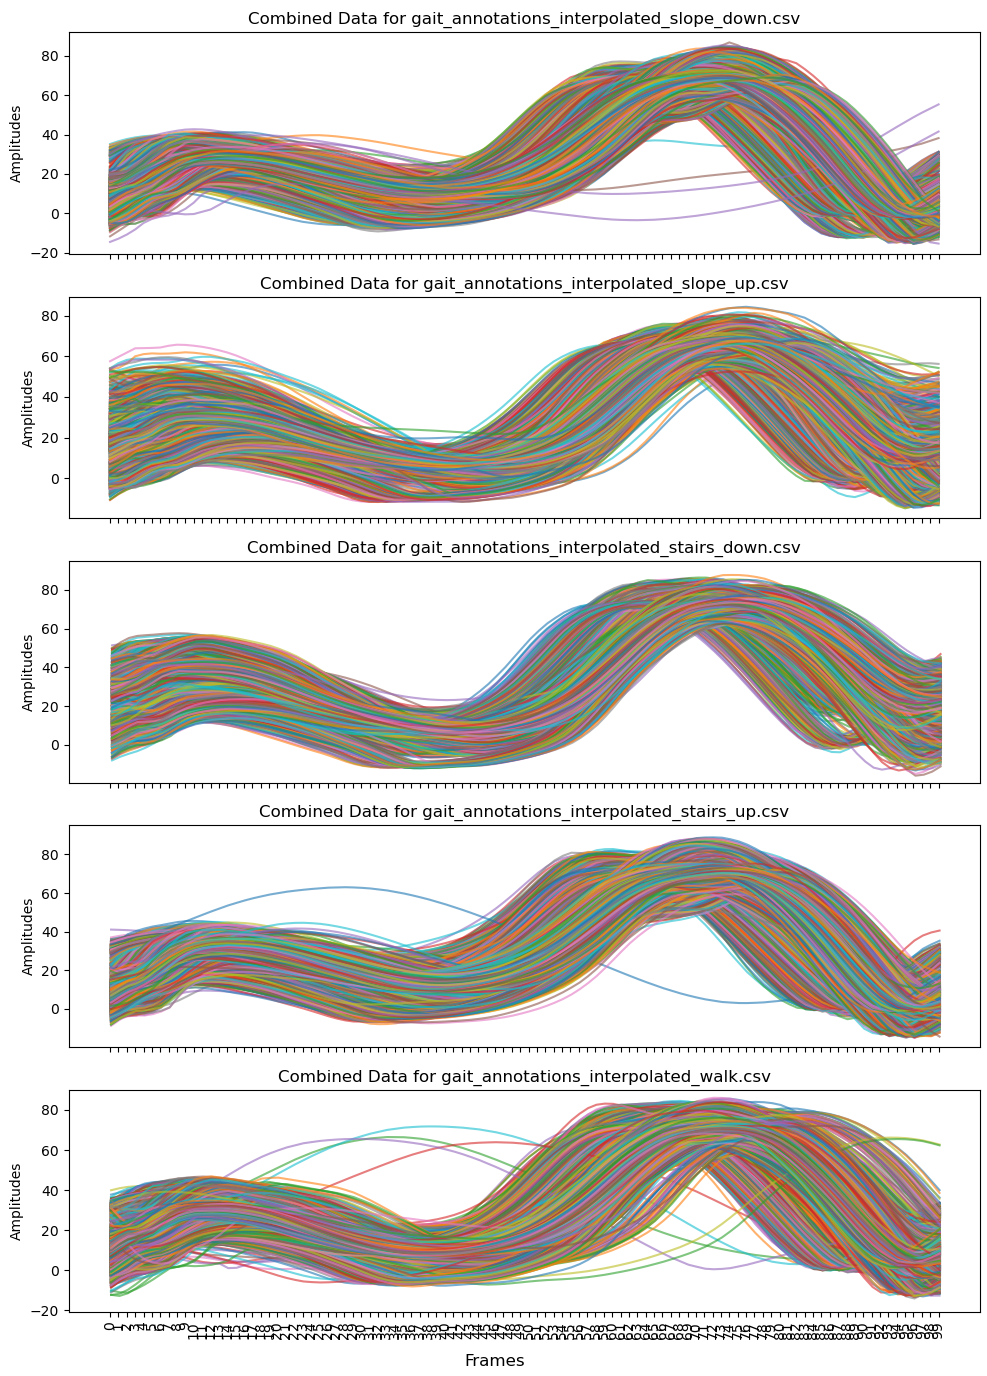
\includegraphics[width=0.95\linewidth]{figures/knee angle sagittal plane curves per gait cycle-per surface.png}
    \caption{Sagittal plane knee angles, normalized to 100\% of the gait cycle, available from the processed IMUs to gauge the success of the gait segmentation strategy.}
    \label{fig:joint_angles}
\end{figure}

\begin{landscape}
    

\begin{figure}[ht]
    \centering
    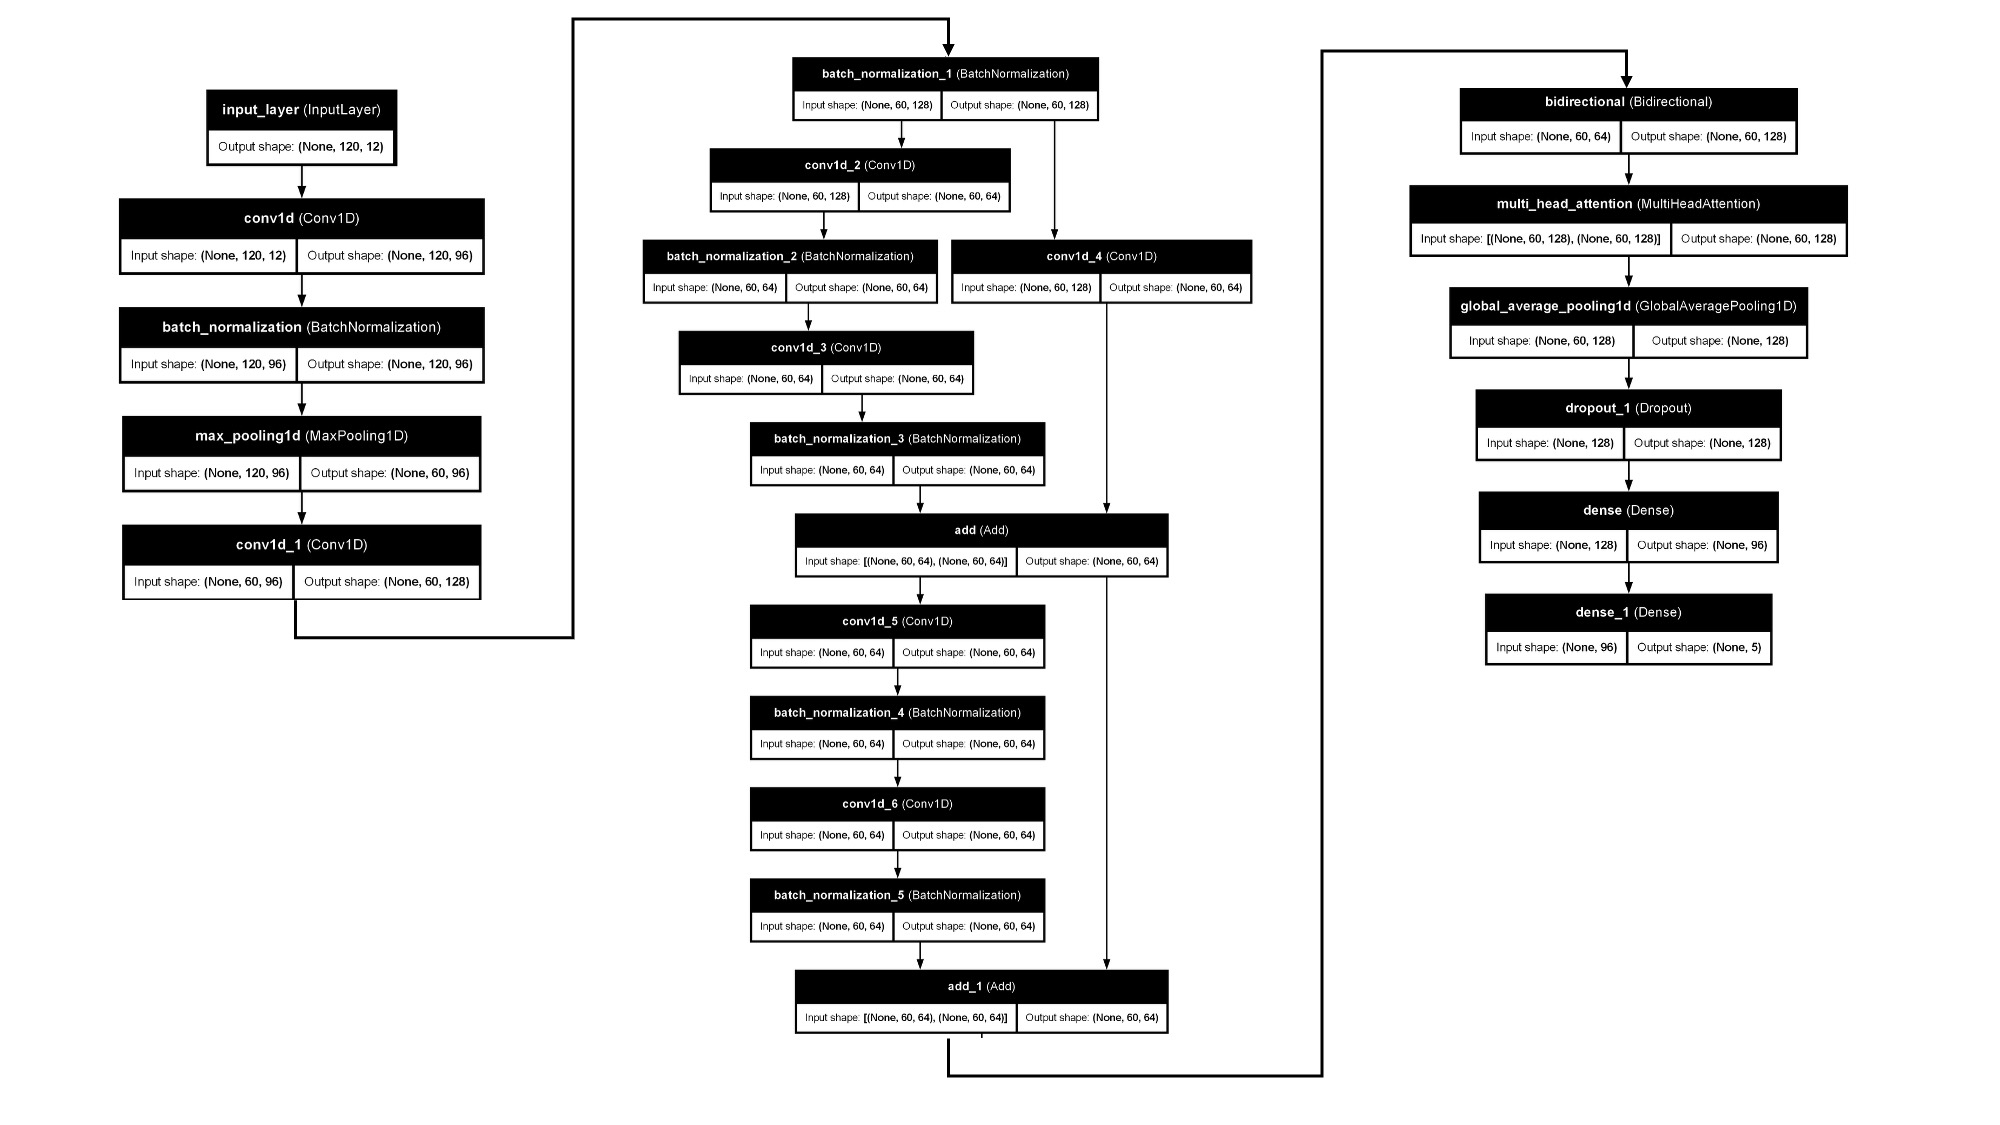
\includegraphics[width=0.95\linewidth]{figures/model_architecture}
    \caption{Model architecture of the deep learning model.}
    \label{fig:model_architecture}
\end{figure}
\end{landscape}

% \begin{figure}
%     \centering
%     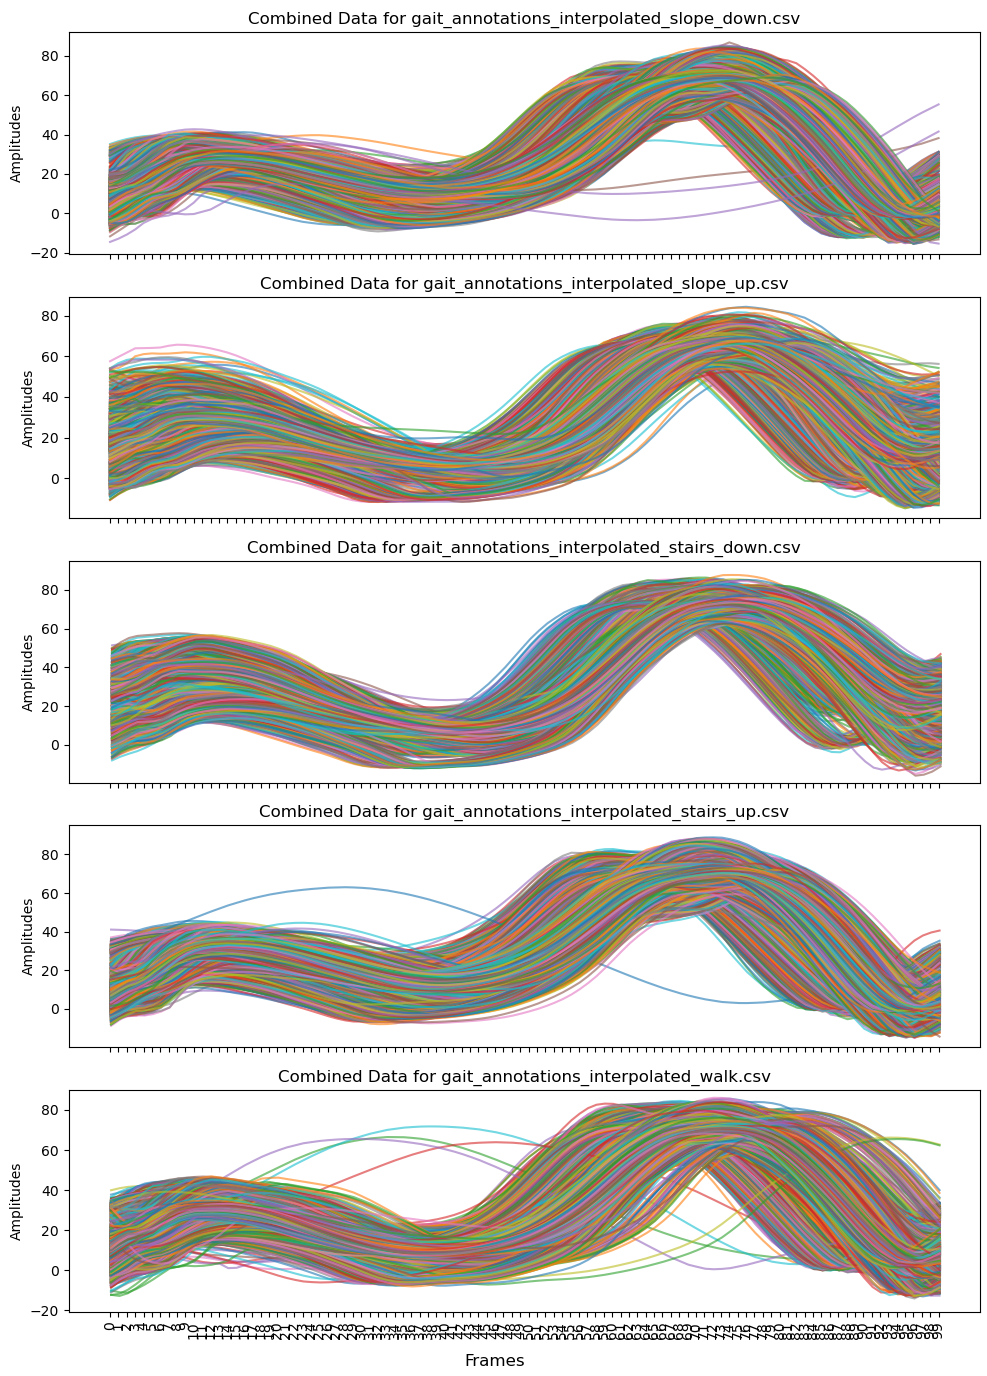
\includegraphics[width=0.95\linewidth]{figures/knee angle sagittal plane curves per gait cycle-per surface.png}
%     \caption{Sagittal plane knee angles, normalized to 100\% of the gait cycle, available from the processed IMUs to gauge the success of the gait segmentation strategy}
%     \label{fig:joint_angles}
% \end{figure}

% \end{document}
